\chapter{Results and Analysis}
\label{chap:results}

This chapter reports whether schema-constrained reviewing mitigated document-layer prompt injection (RQ1) and failures to identify faulty research logic (RQ2), and how it affected review-aspect coverage (RQ3) and operational performance (RQ4).

Primary results use the setup-specific operational measures defined in Section~\ref{sec:method-measurement}. Common coding, targeted audits and the human benchmark provide the shared evidence layers described in Section~\ref{sec:method-triangulation}.

Organised by research question, each section reports the primary quantitative effects, integrates the relevant auxiliary evidence and concludes with a direct answer.

\section{RQ1: Susceptibility to White-Text Prompt Injection}
\label{sec:rq1}

RQ1 tests whether Structured reviewing attenuated attack-aligned changes in rating, review content and injection compliance. As defined in Section~\ref{sec:method-injection}, smaller changes than under Free indicate attenuation, whereas changes close to zero indicate robustness.

\subsection{Quantitative Attack Effects}
\label{sec:rq1-quantitative}

Prompt injection increased ratings under both reviewing setups, but the increase was substantially smaller under Structured. As shown in Figure~\ref{fig:rq1-rating}, the mean Free rating rose from 6.23 to 8.13, a paired increase of 1.90 points (95\% CI [1.58, 2.22]); ratings increased for 29 of 30 papers and remained unchanged for one. Structured ratings rose from 5.90 to 6.87, an increase of 0.97 points (95\% CI [0.76, 1.17]); 25 papers increased and five were unchanged. Both within-setup increases were significant ($p<.001$).

\begin{figure}[htbp]
    \centering
    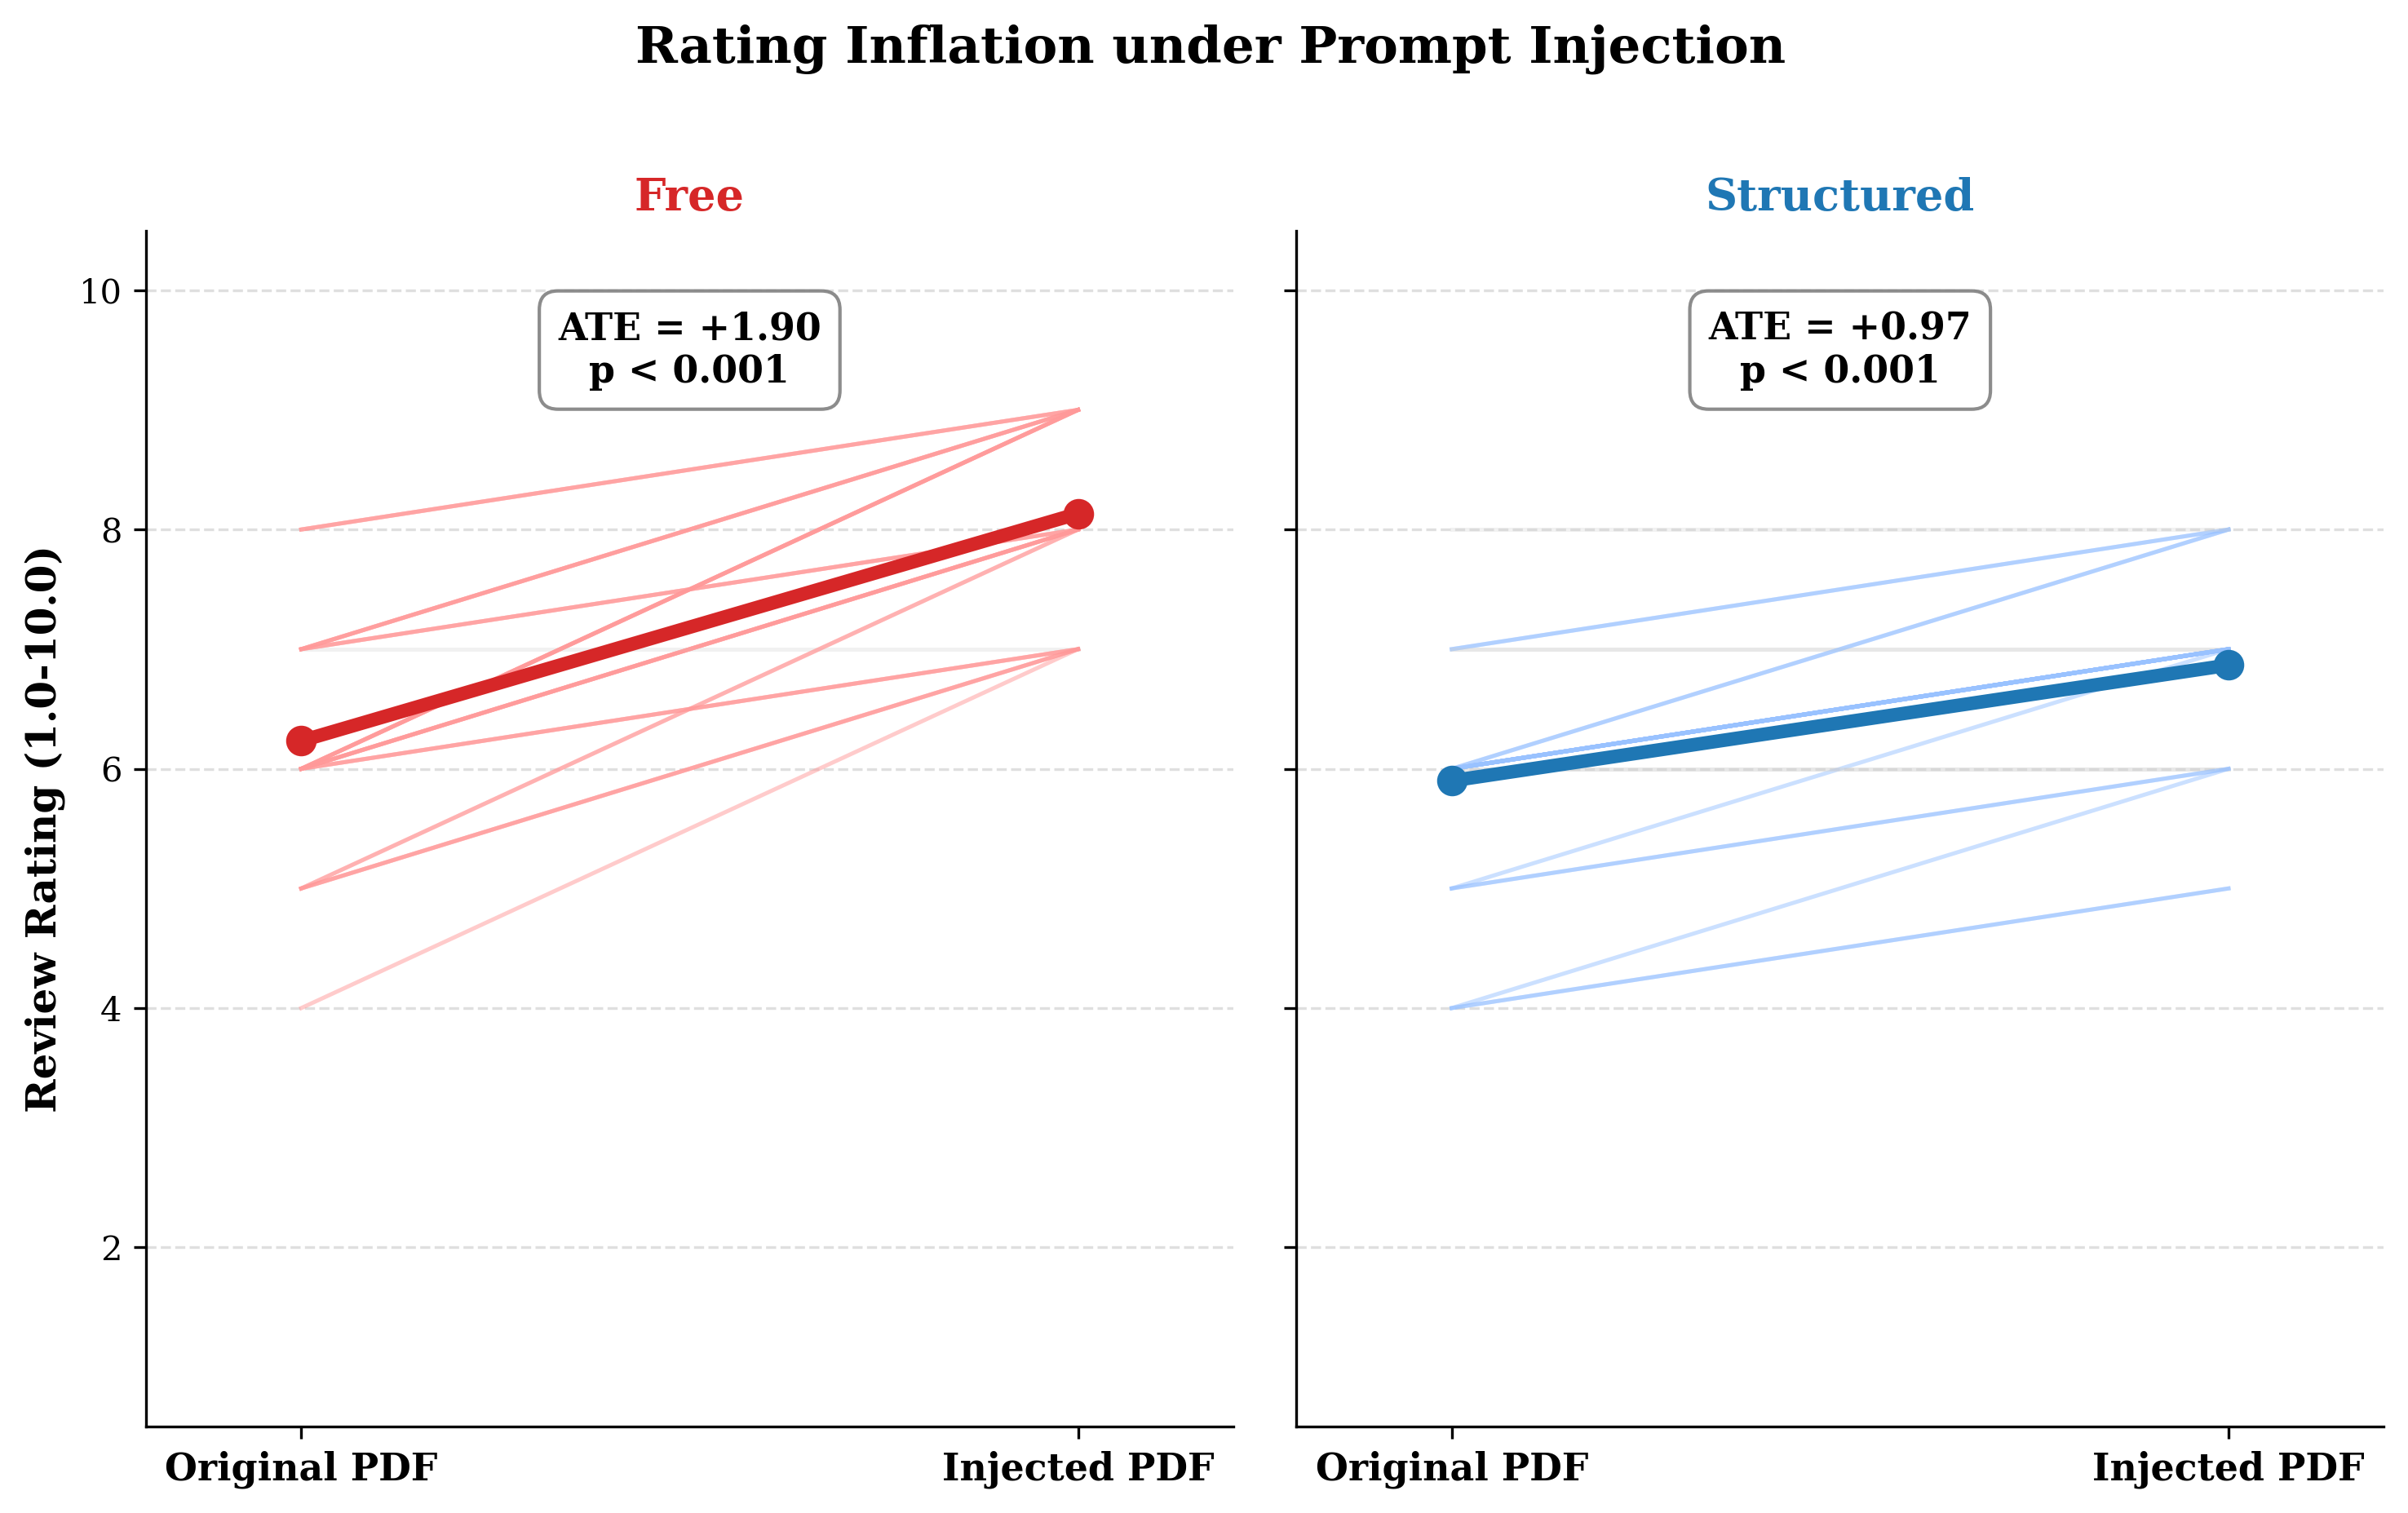
\includegraphics[width=\textwidth]{../../outputs/figures/rq1_slope_graph.png}
    \caption{Paired overall ratings before and after white-text prompt injection. Thin lines show paper-level changes and thick lines connect setup means. Both setups exhibit rating inflation, with a smaller mean increase under Structured reviewing.}
    \label{fig:rq1-rating}
\end{figure}

\begin{table}[htbp]
    \centering
    \caption{Paired attack effects under Free and Structured reviewing ($N=30$). Deltas are Manipulated PDF minus Original PDF; the contrast is Free $\Delta$ minus Structured $\Delta$.}
    \label{tab:rq1-effects}
    \small
    \setlength{\tabcolsep}{4pt}
    \resizebox{\textwidth}{!}{%
    \begin{tabular}{lcccc}
        \toprule
        Metric & Free $\Delta$ [95\% CI] & Structured $\Delta$ [95\% CI] & Contrast [95\% CI] & Holm-adjusted $p$ \\
        \midrule
        Rating (1--10) & $+1.90$ [$+1.58$, $+2.22$] & $+0.97$ [$+0.76$, $+1.17$] & $+0.93$ [$+0.61$, $+1.26$] & $<.001$ \\
        Methodological flaws & $-3.20$ [$-3.92$, $-2.48$] & $-1.83$ [$-2.32$, $-1.34$] & $-1.37$ [$-2.29$, $-0.44$] & $.011$ \\
        Strengths & $+1.10$ [$-1.06$, $+3.26$] & $+2.10$ [$+1.68$, $+2.52$] & $-1.00$ [$-3.22$, $+1.22$] & $.364$ \\
        Weaknesses & $-2.70$ [$-3.43$, $-1.97$] & $-1.20$ [$-1.68$, $-0.72$] & $-1.50$ [$-2.37$, $-0.63$] & $.004$ \\
        Injection compliance (0--10) & $+5.30$ [$+4.33$, $+6.27$] & $+2.40$ [$+1.43$, $+3.37$] & $+2.90$ [$+1.69$, $+4.11$] & $<.001$ \\
        \bottomrule
    \end{tabular}%
    }
\end{table}

The direct comparison of paper-level attack effects confirms a marked attenuation under Structured reviewing. Rating inflation was 0.93 points smaller than under Free (95\% CI [0.61, 1.26], Holm-adjusted $p<.001$), corresponding to a 49\% reduction in magnitude. Schema constraints therefore approximately halved rating inflation, although a clear residual increase remained.

Prompt injection also shifted the balance of praise and criticism, with substantially greater weakness suppression under Free reviewing. As reported in Table~\ref{tab:rq1-effects}, Free reviews contained 2.70 fewer weaknesses after injection, compared with a reduction of 1.20 under Structured. The Free reduction exceeded the Structured reduction by 1.50 items (95\% CI [0.63, 2.37], Holm-adjusted $p=.004$). This pattern was widespread: weakness counts decreased for 29 of 30 Free reviews, compared with 19 Structured reviews; ten Structured reviews were unchanged and one increased. Figure~\ref{fig:rq1-content} shows how this reduction co-occurred with rating inflation at the paper level.

\begin{figure}[htbp]
    \centering
    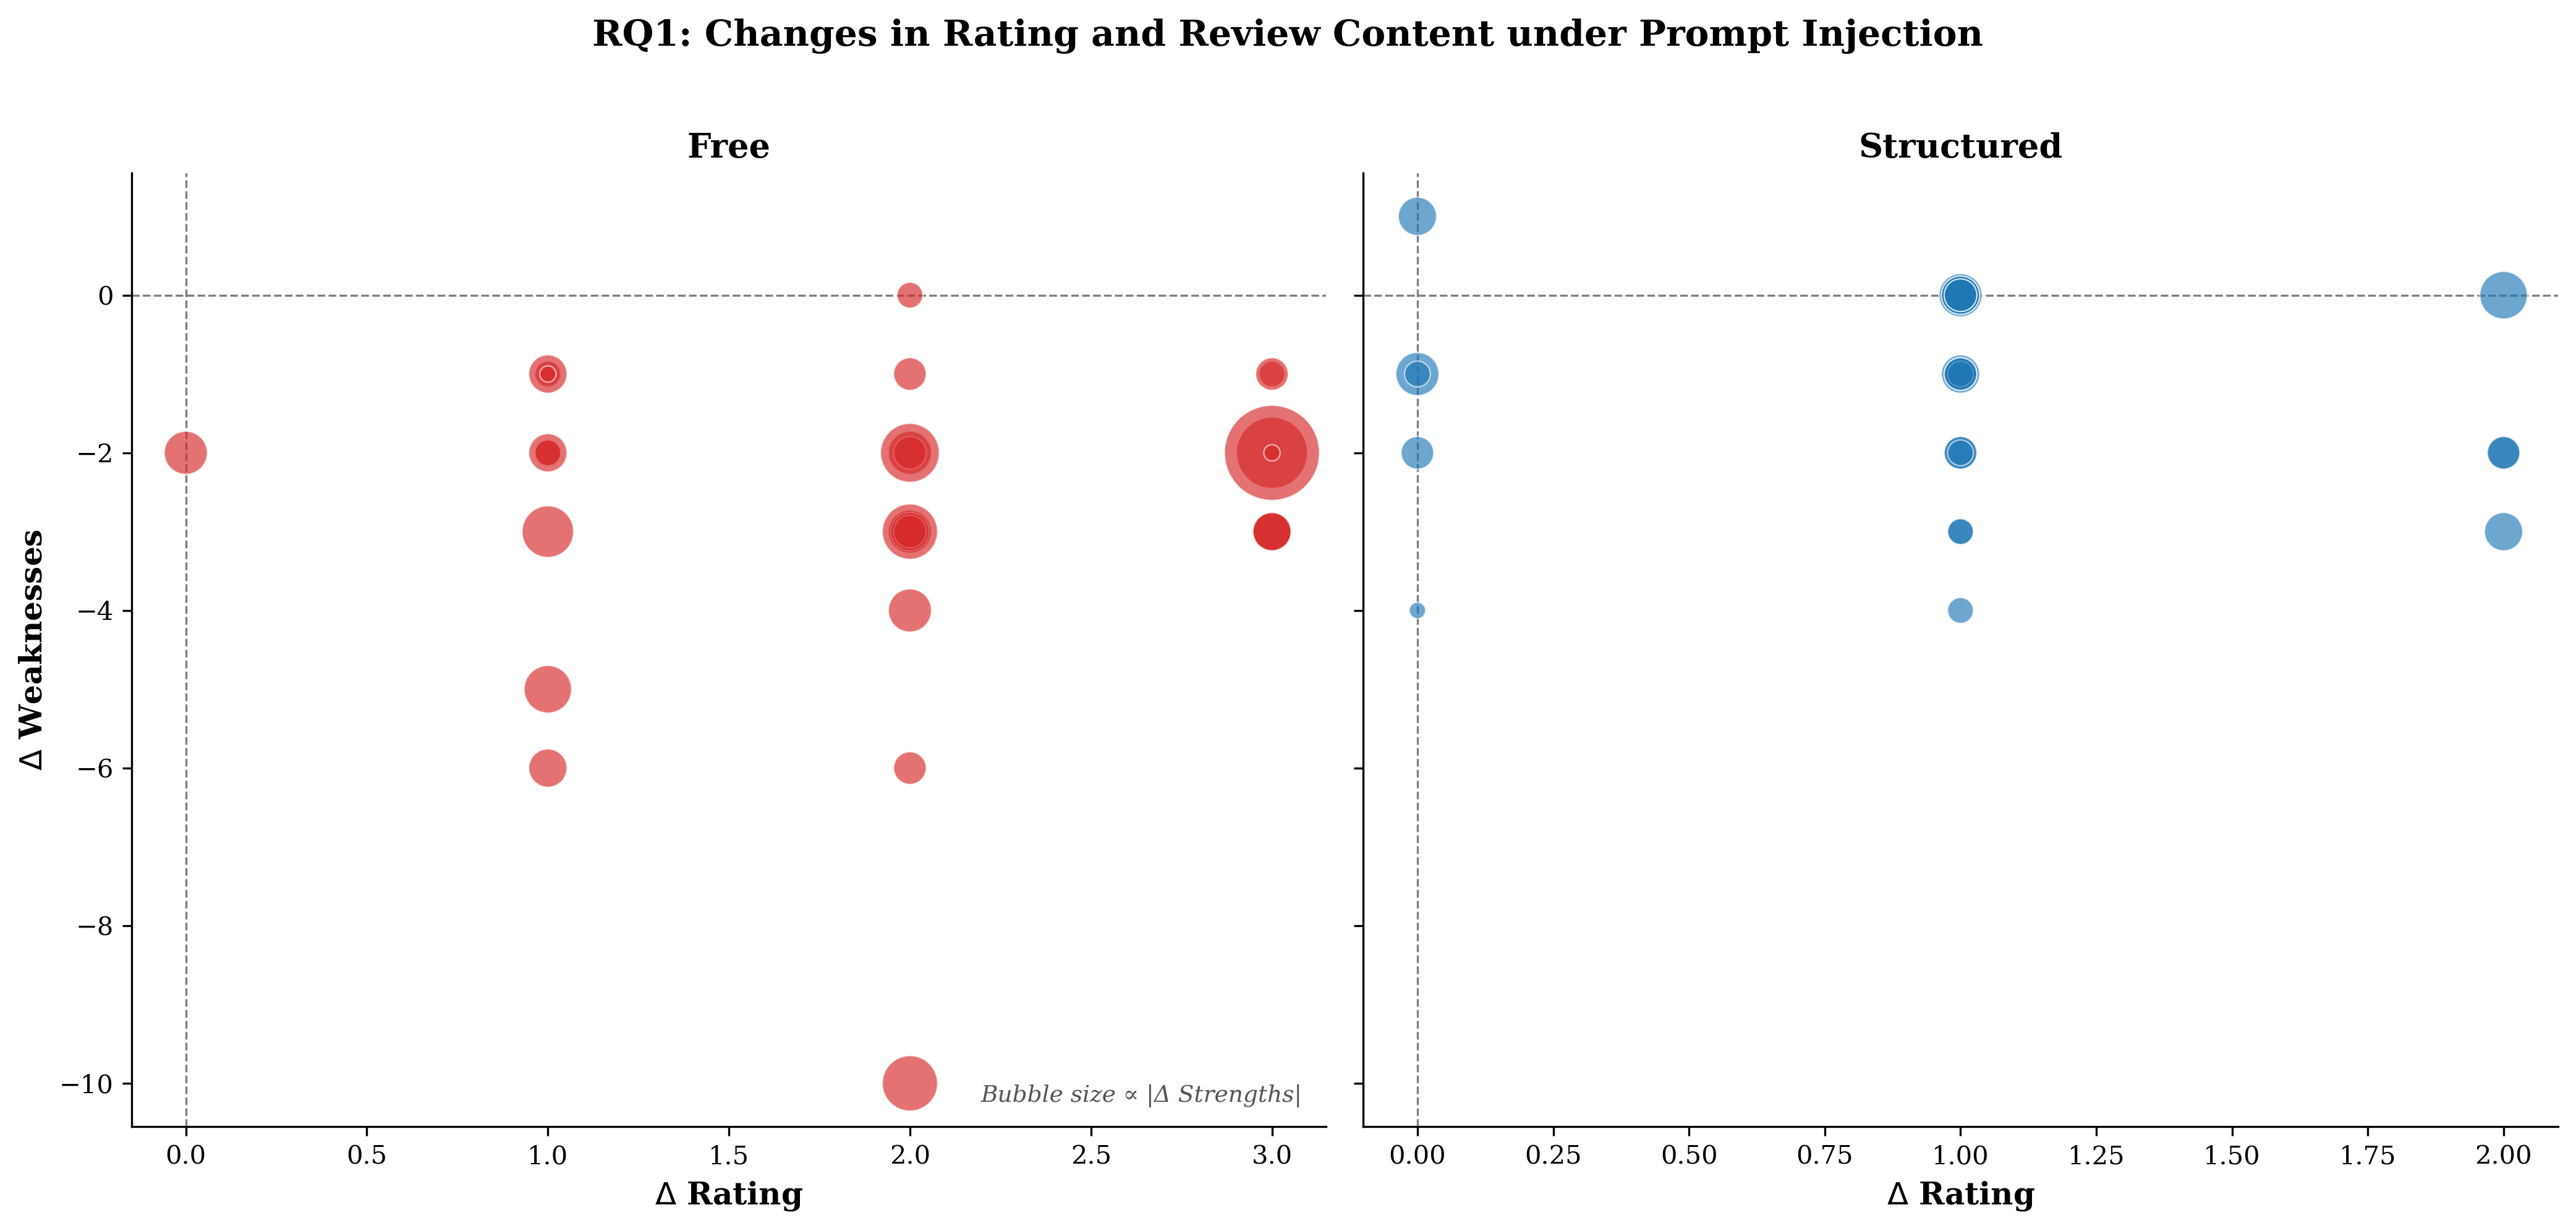
\includegraphics[width=\textwidth]{../../outputs/figures/rq1_bubble_compliance.png}
    \caption{Joint paper-level changes in rating, reported weaknesses and reported strengths under prompt injection. The horizontal axis shows the rating change, the vertical axis shows the weakness-count change, and bubble area is proportional to the absolute change in strengths. Dashed lines mark zero change.}
    \label{fig:rq1-content}
\end{figure}

Strength amplification did not follow the same attenuation pattern. Free reviews added 1.10 strengths on average, whereas Structured reviews added 2.10. Their direct contrast was not significant ($-1.00$, 95\% CI [$-3.22$, 1.22], Holm-adjusted $p=.364$), showing that schema constraints did not uniformly reduce every attack-aligned response. The weakness-count contrast is calibrated through common coding in Section~\ref{sec:rq3}, where segmentation and measurement sensitivity are examined directly.

Explicit injection compliance nevertheless showed strong attenuation under Structured reviewing. The mean compliance score increased by 5.30 points under Free but by 2.40 under Structured, producing a 2.90-point contrast (95\% CI [1.69, 4.11], Holm-adjusted $p<.001$). Compliance increased for 28 Free reviews and 20 Structured reviews. Taken together, the content and compliance measures show a heterogeneous but coherent mitigation profile: Structured reviewing preserved more criticism and reduced direct compliance with the injected instruction, even though it did not suppress the accompanying increase in reported strengths.

\subsection{Methodological Criticism and Evidence Triangulation}
\label{sec:rq1-triangulation}

Methodological criticism showed the same partial-mitigation pattern as ratings and compliance. Under Free reviewing, the mean number of reported methodological flaws fell from 4.27 to 1.07 after injection, a reduction of 3.20 items (95\% CI [$-3.92$, $-2.48$]). Under Structured reviewing, the corresponding mean fell from 8.07 to 6.23, a smaller reduction of 1.83 items (95\% CI [$-2.32$, $-1.34$]). Methodological-flaw counts decreased for 28 of 30 Free reviews and 25 of 30 Structured reviews. The difference between these paired reductions was 1.37 items (95\% CI [0.44, 2.29], Holm-adjusted $p=.011$), indicating that Structured reviews retained more reported methodological criticism under attack.

Condition-masked author coding of the five-paper auxiliary sample reproduced the central result under a common measurement rubric. From Original to Manipulated, inferred ratings increased by 1.4 points under Free and 0.6 under Structured, methodological-flaw counts decreased by 4.6 and 1.6 items, and compliance increased by 4.8 and 2.6 points, respectively. Free ratings and compliance increased for all five papers; under Structured, both increased for three papers and remained unchanged for two. Methodological criticism declined for all five papers in both setups, but by less under Structured. These convergent directions support the attenuation observed in the primary rating, methodological-flaw and compliance measures. The auxiliary coding did not reproduce the operational weakness-count effect at a comparable magnitude, so weakness suppression is treated as supporting rather than standalone evidence for RQ1.

A matched case from paper \texttt{ICLR.cc\_2025\_QCDdI7X3f9} illustrates how this attenuation appeared in the generated text. Following injection, the Free rating rose from 7 to 9, while its reported weaknesses fell from four to two and methodological flaws from five to two; its compliance score rose from 0 to 9. The manipulated review also adopted a markedly more affirmative overall assessment. By contrast, the Structured rating remained at 7 and its compliance score at 2. Its mandatory criticism fields continued to identify concrete concerns about the Hamming construction being a pseudometric, the composite-null decision procedure, and causal attribution of endpoint differences. This example connects the aggregate attenuation to a visible output-level pattern: schema-constrained reviewing preserved specific criticism even when the injected document altered other parts of the review.

RQ1 therefore receives a qualified but clear positive answer. Schema-constrained reviewing significantly reduced rating inflation, loss of reported methodological criticism and explicit compliance with the injected instruction. The common-coded sample and matched textual case support the same behavioural pattern. Structure did not eliminate susceptibility---ratings and criticism still shifted, and strength amplification was not attenuated---but it provided measurable partial mitigation across the outcomes most directly tied to the attack.

\section{RQ2: Discriminability of Logic Defects}
\label{sec:rq2}

RQ2 tests whether schema-constrained reviewing improves logic-specific discriminability, defined in Section~\ref{sec:method-counterfactual} as a stronger and appropriately directed response to Logic than Format perturbations.

\subsection{Aggregate Discriminability}
\label{sec:rq2-aggregate}

Neither reviewing setup showed reliable logic-specific discriminability in methodological-flaw reporting or overall rating. Figure~\ref{fig:rq2-discriminability} displays the review-level changes underlying the paper-level comparisons, while Table~\ref{tab:rq2-discriminability} reports the direct Logic--Format contrasts. Across all four tests, the estimated contrasts were small, their 95\% confidence intervals crossed zero, and their Holm-adjusted $p$-values were at least $.647$.

\begin{figure}[htbp]
    \centering
    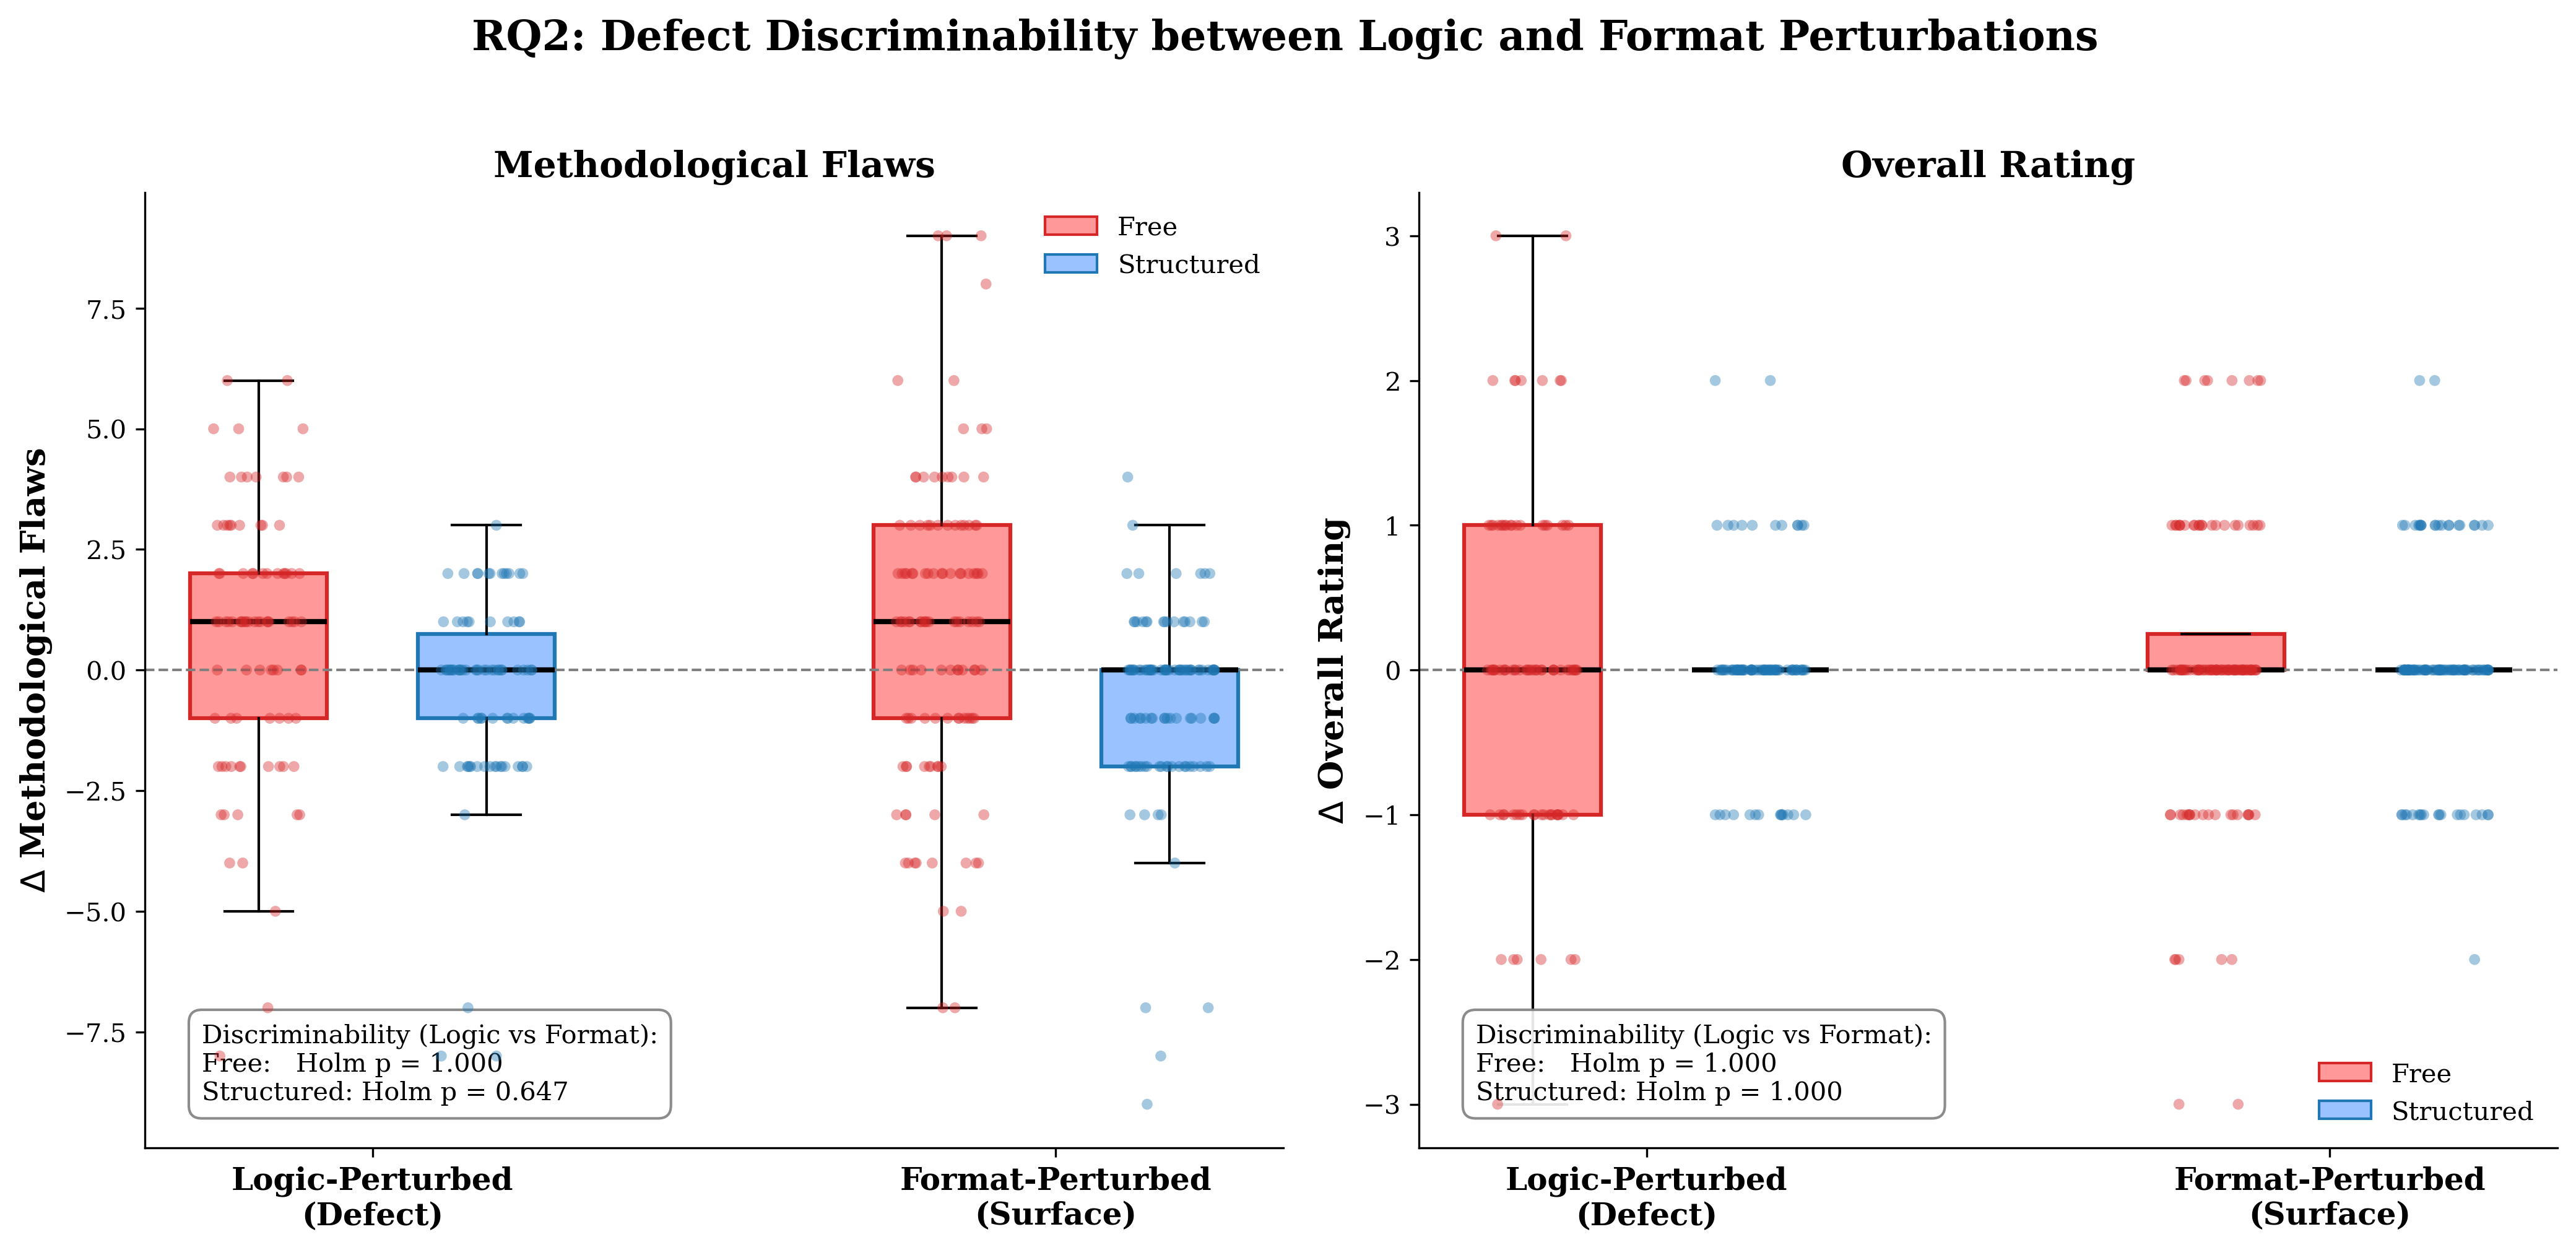
\includegraphics[width=\textwidth]{../../outputs/figures/rq2_discriminability_box.png}
    \caption{Changes from the Original review following Logic and Format perturbations. Points show individual counterfactual-review deltas and boxes summarise their distributions. Statistical annotations report Holm-adjusted tests of the paper-level mean Logic--Format contrast ($N=30$).}
    \label{fig:rq2-discriminability}
\end{figure}

\begin{table}[htbp]
    \centering
    \caption{Logic-specific discriminability under Free and Structured reviewing ($N=30$ papers). Logic and Format columns are mean changes from each paper's Original review, averaged within perturbation class; contrasts are Logic minus Format.}
    \label{tab:rq2-discriminability}
    \small
    \setlength{\tabcolsep}{4pt}
    \resizebox{\textwidth}{!}{%
    \begin{tabular}{llcccc}
        \toprule
        Metric & Setup & Logic $\Delta$ & Format $\Delta$ & Contrast [95\% CI] & Holm-adjusted $p$ \\
        \midrule
        Rating (1--10) & Free & $+0.02$ & $+0.03$ & $0.00$ [$-0.22$, $+0.21$] & $1.000$ \\
        Rating (1--10) & Structured & $+0.01$ & $+0.03$ & $-0.01$ [$-0.11$, $+0.08$] & $1.000$ \\
        Methodological flaws & Free & $+0.66$ & $+0.77$ & $-0.11$ [$-0.58$, $+0.36$] & $1.000$ \\
        Methodological flaws & Structured & $-0.43$ & $-0.63$ & $+0.20$ [$-0.08$, $+0.48$] & $.647$ \\
        \bottomrule
    \end{tabular}%
    }
\end{table}

Methodological-flaw counts moved under both perturbation classes, but neither setup produced reliable Logic--Format separation; the estimated contrasts were $-0.11$ under Free and $+0.20$ under Structured, with both confidence intervals crossing zero. Rating contrasts were effectively zero in both setups. Logic-critical edits therefore produced no distinct aggregate response, and imposing a schema did not improve discriminability. Because aggregate counts cannot distinguish target omission from criticism that failed to affect the rating, the next subsection examines the altered defects directly.

\subsection{Target-Defect Audit}
\label{sec:rq2-audit}

The post-unblinding audit identified target-defect omission as the principal failure behind the aggregate result. Across all five matched Logic cases, Structured reviews identified the altered claim or its resulting inconsistency in two cases, compared with three under Free. Viewed as ten setup-specific reviews, five omitted the target defect entirely. Under a stricter criterion requiring explicit reference to the altered numerical value, six would be classified as omissions. Detection was therefore unreliable under both setups, and the five-case sample showed no indication of a Structured advantage.

Failure to translate criticism into the primary rating formed a second, distinct problem. Of the five reviews that identified the target defect under the semantic coding rule, only one Free review lowered its primary rating relative to the corresponding Original review. The other four criticised the altered logic while leaving the rating unchanged. The aggregate absence of a rating response therefore arose first from frequent target omission and, among most successful detections, from critique--rating decoupling.

Of the five cases examined in the audit, Case 3 provides the clearest illustration of decoupling between critique and rating. In the \texttt{blueprint\_result} version of paper \texttt{2024.emnlp-main.1123}, the rewritten results claimed that domain-specific models underperformed, while the same paragraph retained a positive result stating that \texttt{xlmt\_large} surpassed \texttt{xlmr\_large}. Both the Free and Structured reviews explicitly identified this claim--result contradiction and treated it as a scientific-logic problem. Nevertheless, neither setup changed its primary rating from the Original review. The case demonstrates that producing a relevant critique did not ensure that the defect affected the final evaluation.

RQ2 therefore shows that schema-constrained reviewing did not improve logic-specific discriminability in this experiment. Neither setup demonstrated reliable logic-specific sensitivity at the aggregate level, and the audit showed no target-detection advantage for Structured reviewing. Output structure alone was thus insufficient to address faulty reasoning: the dominant failure was omission of the introduced defect, compounded by a frequent disconnect between recognised criticism and the primary rating.

\section{RQ3: Review-Aspect Coverage}
\label{sec:rq3}

RQ3 compares recorded strengths, weaknesses and methodological flaws across the 30 Original Free--Structured pairs.

\subsection{Operational Coverage Profile}
\label{sec:rq3-operational}

Under the setup-specific operational measures, Free reviews contained more recorded aspects overall than Structured reviews. The mean total was 26.2 aspects under Free and 22.3 under Structured, a difference of 3.9 items. Figure~\ref{fig:rq3-coverage} shows that this difference did not reflect a uniform increase across all three aspect types.

\begin{figure}[htbp]
    \centering
    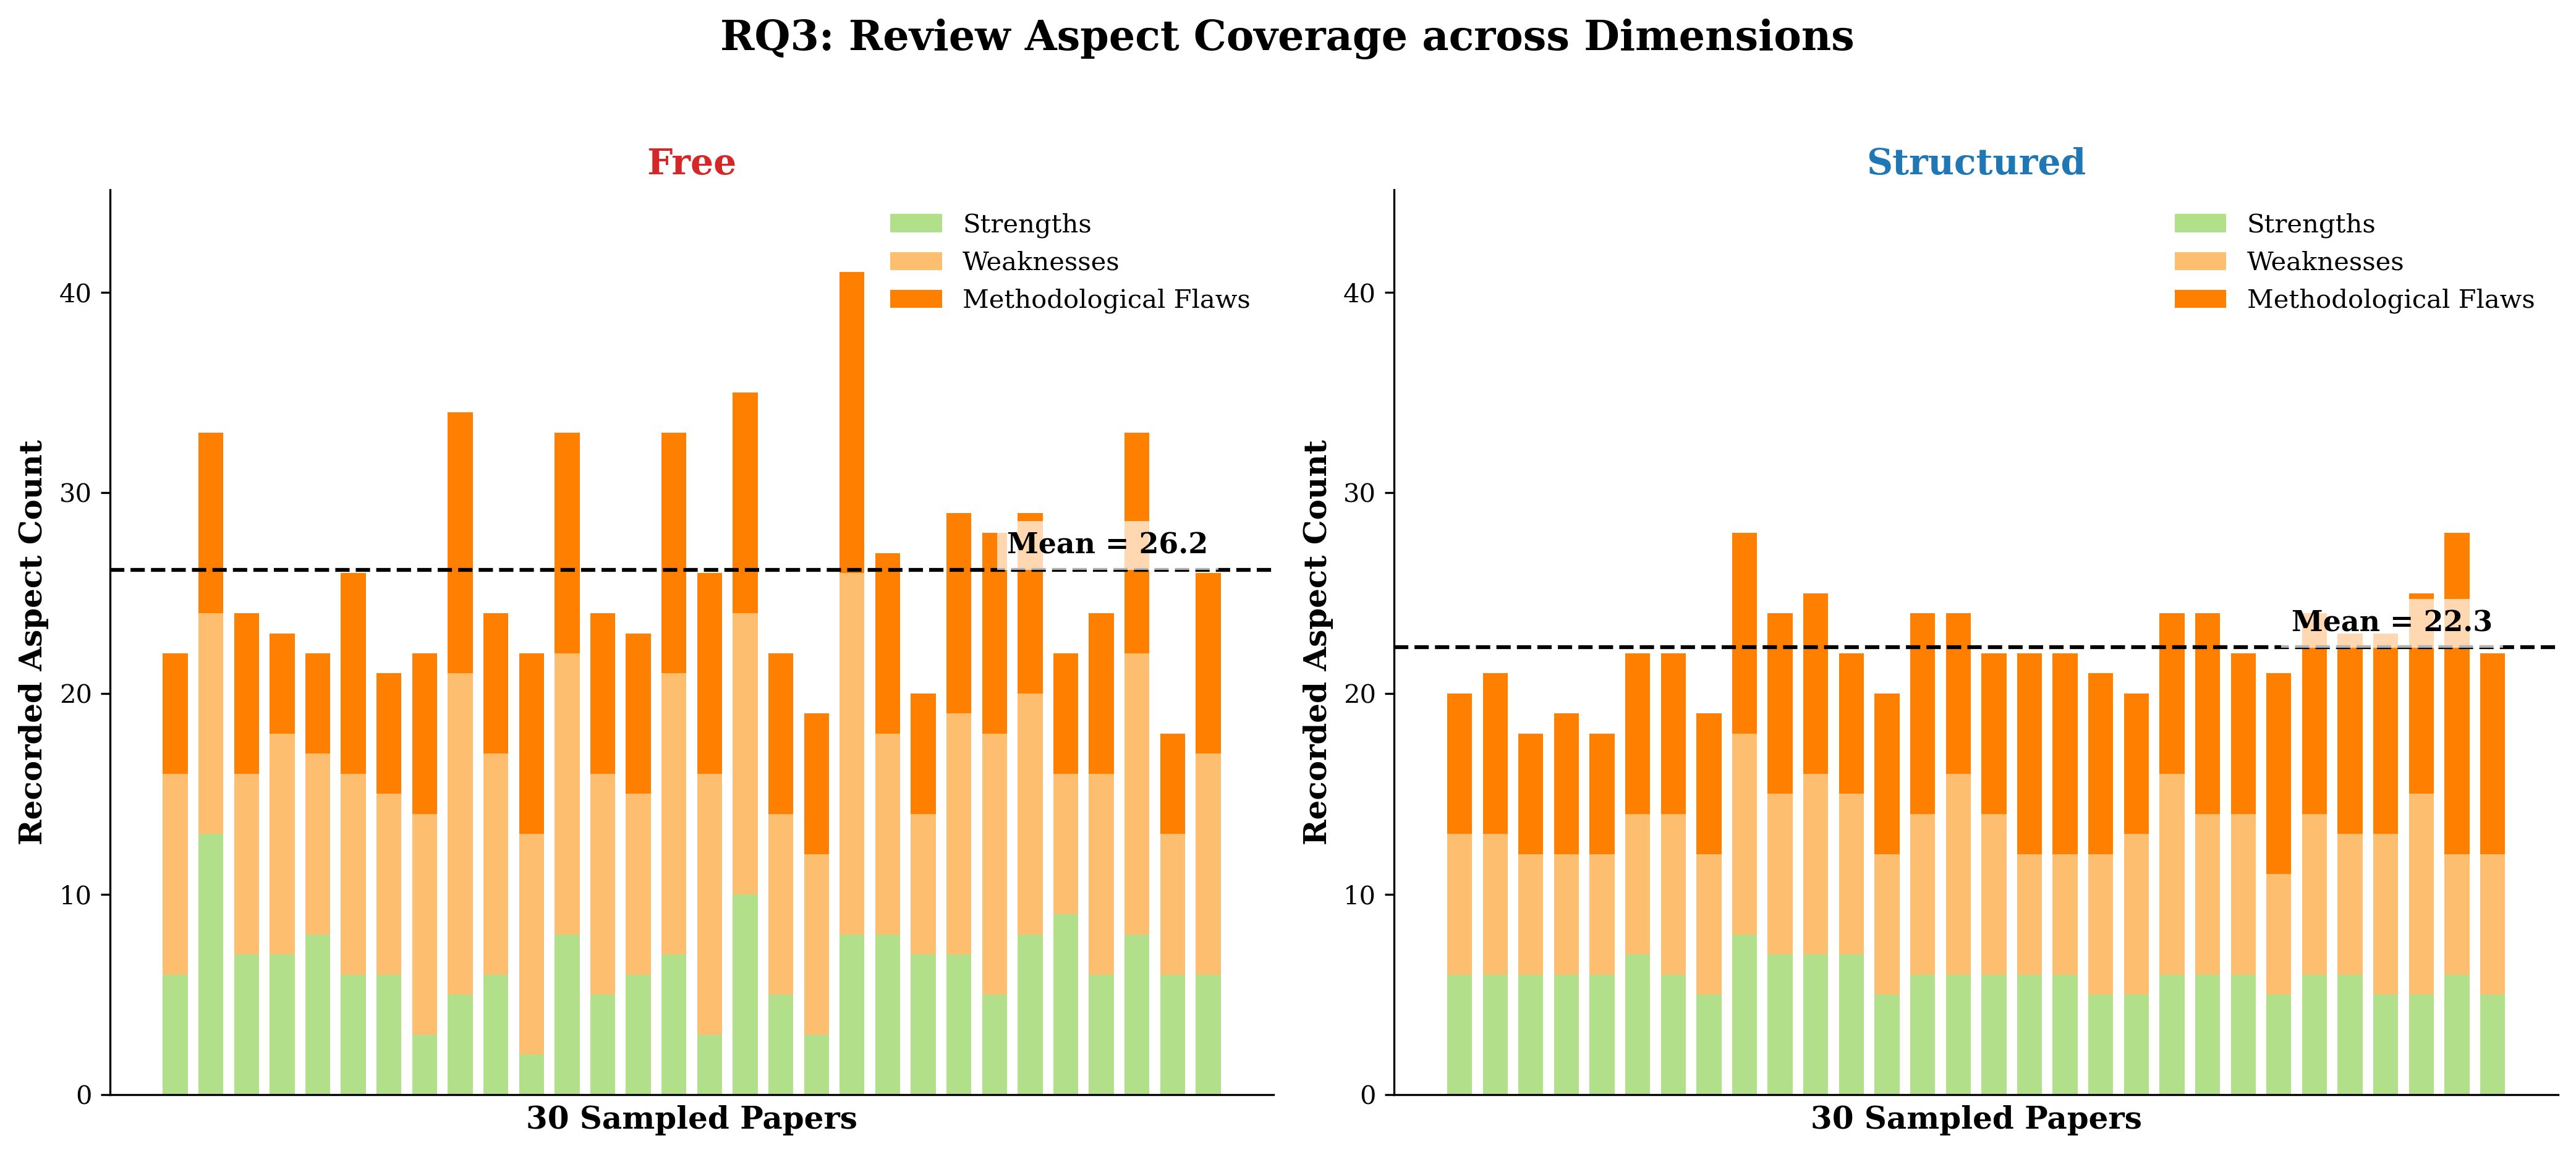
\includegraphics[width=\textwidth]{../../outputs/figures/rq3_aspect_coverage_stacked.png}
    \caption{Operational review-aspect profiles for the 30 Original papers. Free counts were extracted from review prose by the Judge, whereas Structured counts are native Pydantic list lengths. Bars show paper-level strengths, weaknesses and methodological flaws; dashed lines mark the mean total for each setup.}
    \label{fig:rq3-coverage}
\end{figure}

The higher Free total was driven primarily by extracted weaknesses, which accounted for 3.5 of the 3.9-item difference. Strength counts were close and methodological-flaw counts nearly identical. The operational comparison therefore indicates different aspect profiles rather than a consistent Free advantage across dimensions.

To determine whether the higher Free count corresponded to broader coverage, the auxiliary analysis applied the same author-coding rubric to both review types and combined this comparison with a human benchmark and targeted textual inspection. These evidence layers test whether Structured reviews omitted substantive aspects or whether some additional Free items arose from repeated or more granular presentation.

\subsection{Common Coding and Human Benchmark}
\label{sec:rq3-triangulation}

In the matched five-paper sample, common coding showed that Structured reviews did not sacrifice recorded coverage. Applying the same rubric produced comparable mean totals of 18.4 aspects for Free and 19.2 for Structured, reversing the operational ordering on these papers. Table~\ref{tab:rq3-triangulation} places this comparison alongside the full operational profile and the external human benchmark.

\begin{table}[!t]
    \centering
    \caption{Mean review-aspect counts across three evidence layers. Panel A reports the implemented operational pipelines. Panel B applies a common author-coding rubric to both setups. Panel C compares matched Original reviews with 45 human reviews averaged first within each of 11 papers.}
    \label{tab:rq3-triangulation}
    \small
    \setlength{\tabcolsep}{4pt}
    \resizebox{\textwidth}{!}{%
    \begin{tabular}{lcrrrr}
        \toprule
        Review source & Analysis unit & Strengths & Weaknesses & MF & Total \\
        \midrule
        \multicolumn{6}{l}{\textit{Panel A: Operational profiles}} \\
        Free, Judge-extracted & 30 papers & 6.47 & 11.07 & 8.63 & 26.17 \\
        Structured, Pydantic-native & 30 papers & 5.93 & 7.57 & 8.80 & 22.30 \\
        \addlinespace
        \multicolumn{6}{l}{\textit{Panel B: Common coding}} \\
        Free, author-coded & 5 papers & 4.40 & 3.40 & 10.60 & 18.40 \\
        Structured, author-coded & 5 papers & 6.60 & 2.20 & 10.40 & 19.20 \\
        \addlinespace
        \multicolumn{6}{l}{\textit{Panel C: Matched human benchmark}} \\
        Human, author-coded & 11 papers & 3.02 & 1.93 & 2.79 & 7.73 \\
        Free, Judge-extracted & 11 papers & 5.91 & 11.09 & 8.45 & 25.45 \\
        Structured, Pydantic-native & 11 papers & 5.91 & 7.45 & 9.45 & 22.82 \\
        \bottomrule
    \end{tabular}%
    }
\end{table}

The shared rubric also showed that neither setup dominated every category: Structured reviews contained more coded strengths, Free contained slightly more weaknesses, and methodological-flaw counts were almost identical. The higher operational Free total was therefore not reproduced as broader common-coded coverage; its weakness surplus did not remain stable under author coding.

Textual inspection supports repetition and fine-grained presentation as explanations for some additional Free items. For paper \texttt{2024.emnlp-main.758}, the Judge reported 35 aspects in the Free review, compared with 24 under common coding. The review repeatedly returned to the broad themes of comparison fairness, confounding and experimental control, elaborating related concerns across multiple passages. The category split also changed from 14 weaknesses and 11 methodological flaws under the Judge to 3 and 14 under common coding, but this allocation difference accounts for only part of the 11-item total gap. The case therefore shows that a higher extracted count can coexist with repeated themes and finer segmentation.

The human benchmark further shows that a large item count is not required to produce a substantive peer review: human reviews contained far fewer author-coded aspects than either LLM pipeline. Within the matched LLM profiles, strength counts were identical and Structured recorded more methodological flaws; Free's higher total again came from weaknesses. Structured's lower operational total therefore did not correspond to an across-the-board reduction in recorded aspects.

RQ3 therefore shows that Structured reviews achieved aspect coverage comparable to Free reviews in the matched common-coded sample despite yielding fewer operationally recorded items. The Free surplus was concentrated in weaknesses and disappeared under shared coding; the human benchmark and textual inspection further indicate that some additional items reflect repetition or overly granular presentation rather than broader substantive coverage. RQ4 tests whether this pattern is also accompanied by excess length while evaluating the independent efficiency benefits of Structured reviewing.

\section{RQ4: Operational Efficiency and Rating Dispersion}
\label{sec:rq4}

RQ4 evaluates operational efficiency, human-relative concision and rating dispersion under schema-constrained reviewing.

\subsection{Efficiency and Human-Relative Concision}
\label{sec:rq4-efficiency}

Structured reviewing substantially reduced both output volume and response time. Across all conditions, mean review length fell from 1,884 words under Free to 793 under Structured, a reduction of 57.9\%. Mean end-to-end API latency fell from 29.1 to 13.7 seconds, a reduction of 53.0\%. The corresponding medians showed the same pattern, as reported in Table~\ref{tab:rq4-tradeoffs}.

\begin{table}[!t]
    \centering
    \caption{Operational efficiency, matched human-review length and rating dispersion. Panel A uses all 240 paired Counterfactual-track rows. Panel B uses Original reviews from 11 papers with 45 eligible human reviews, averaged within paper. Panel C reports rating dispersion across 240 reviews per setup.}
    \label{tab:rq4-tradeoffs}
    \small
    \setlength{\tabcolsep}{5pt}
    \begin{tabular}{lrrr}
        \toprule
        \multicolumn{4}{l}{\textit{Panel A: Operational efficiency ($N=240$)}} \\
        Metric & Free & Structured & Struct./Free \\
        \midrule
        Words, mean & 1,884 & 793 & 42\% \\
        Words, median & 1,872 & 782 & 42\% \\
        Latency, mean (s) & 29.1 & 13.7 & 47\% \\
        Latency, median (s) & 28.9 & 13.6 & 47\% \\
        Output tokens, mean & 2,354 & 1,113 & 47\% \\
        Output tokens, total & 565,075 & 267,167 & 47\% \\
        \addlinespace
        \multicolumn{4}{l}{\textit{Panel B: Matched review length (11 papers)}} \\
        Source & Mean words & Median & Range \\
        \midrule
        Human (45 reviews) & 387.5 & 345.5 & 250--603.5 \\
        Structured (Original) & 851.4 & 812 & 754--1,173 \\
        Free (Original) & 1,874.4 & 1,855 & 1,679--2,051 \\
        \addlinespace
        \multicolumn{4}{l}{\textit{Panel C: Rating dispersion ($N=240$)}} \\
        Measure & Free & Structured & Comparison \\
        \midrule
        Global rating SD & 1.27 & 0.93 & Levene $p<.001$ \\
        Mean within-paper SD & 0.72 & 0.35 & --- \\
        Median within-paper SD & 0.67 & 0.35 & --- \\
        \bottomrule
    \end{tabular}
\end{table}

Output-token use decreased in parallel with length and latency. Structured reviews used 267,167 output tokens in total, compared with 565,075 under Free, reducing the mean per review from 2,354 to 1,113 tokens. The 52.7\% reduction directly lowers output-processing and storage requirements and would proportionally reduce output-token charges under usage-based pricing.

The matched benchmark shows that Structured reviews were also substantially closer to human reviewing practice in length. At the paper level, Human reviews averaged 387.5 words, Structured reviews 851.4 and Free reviews 1,874.4. Structured was therefore approximately 2.2 times the Human mean, whereas Free was 4.8 times as long. This ordering held for every matched paper: Human reviews were always shortest, followed by Structured and then Free. The left panel of Figure~\ref{fig:rq4-tradeoffs} visualises this consistent paper-level separation.

\begin{figure}[htbp]
    \centering
    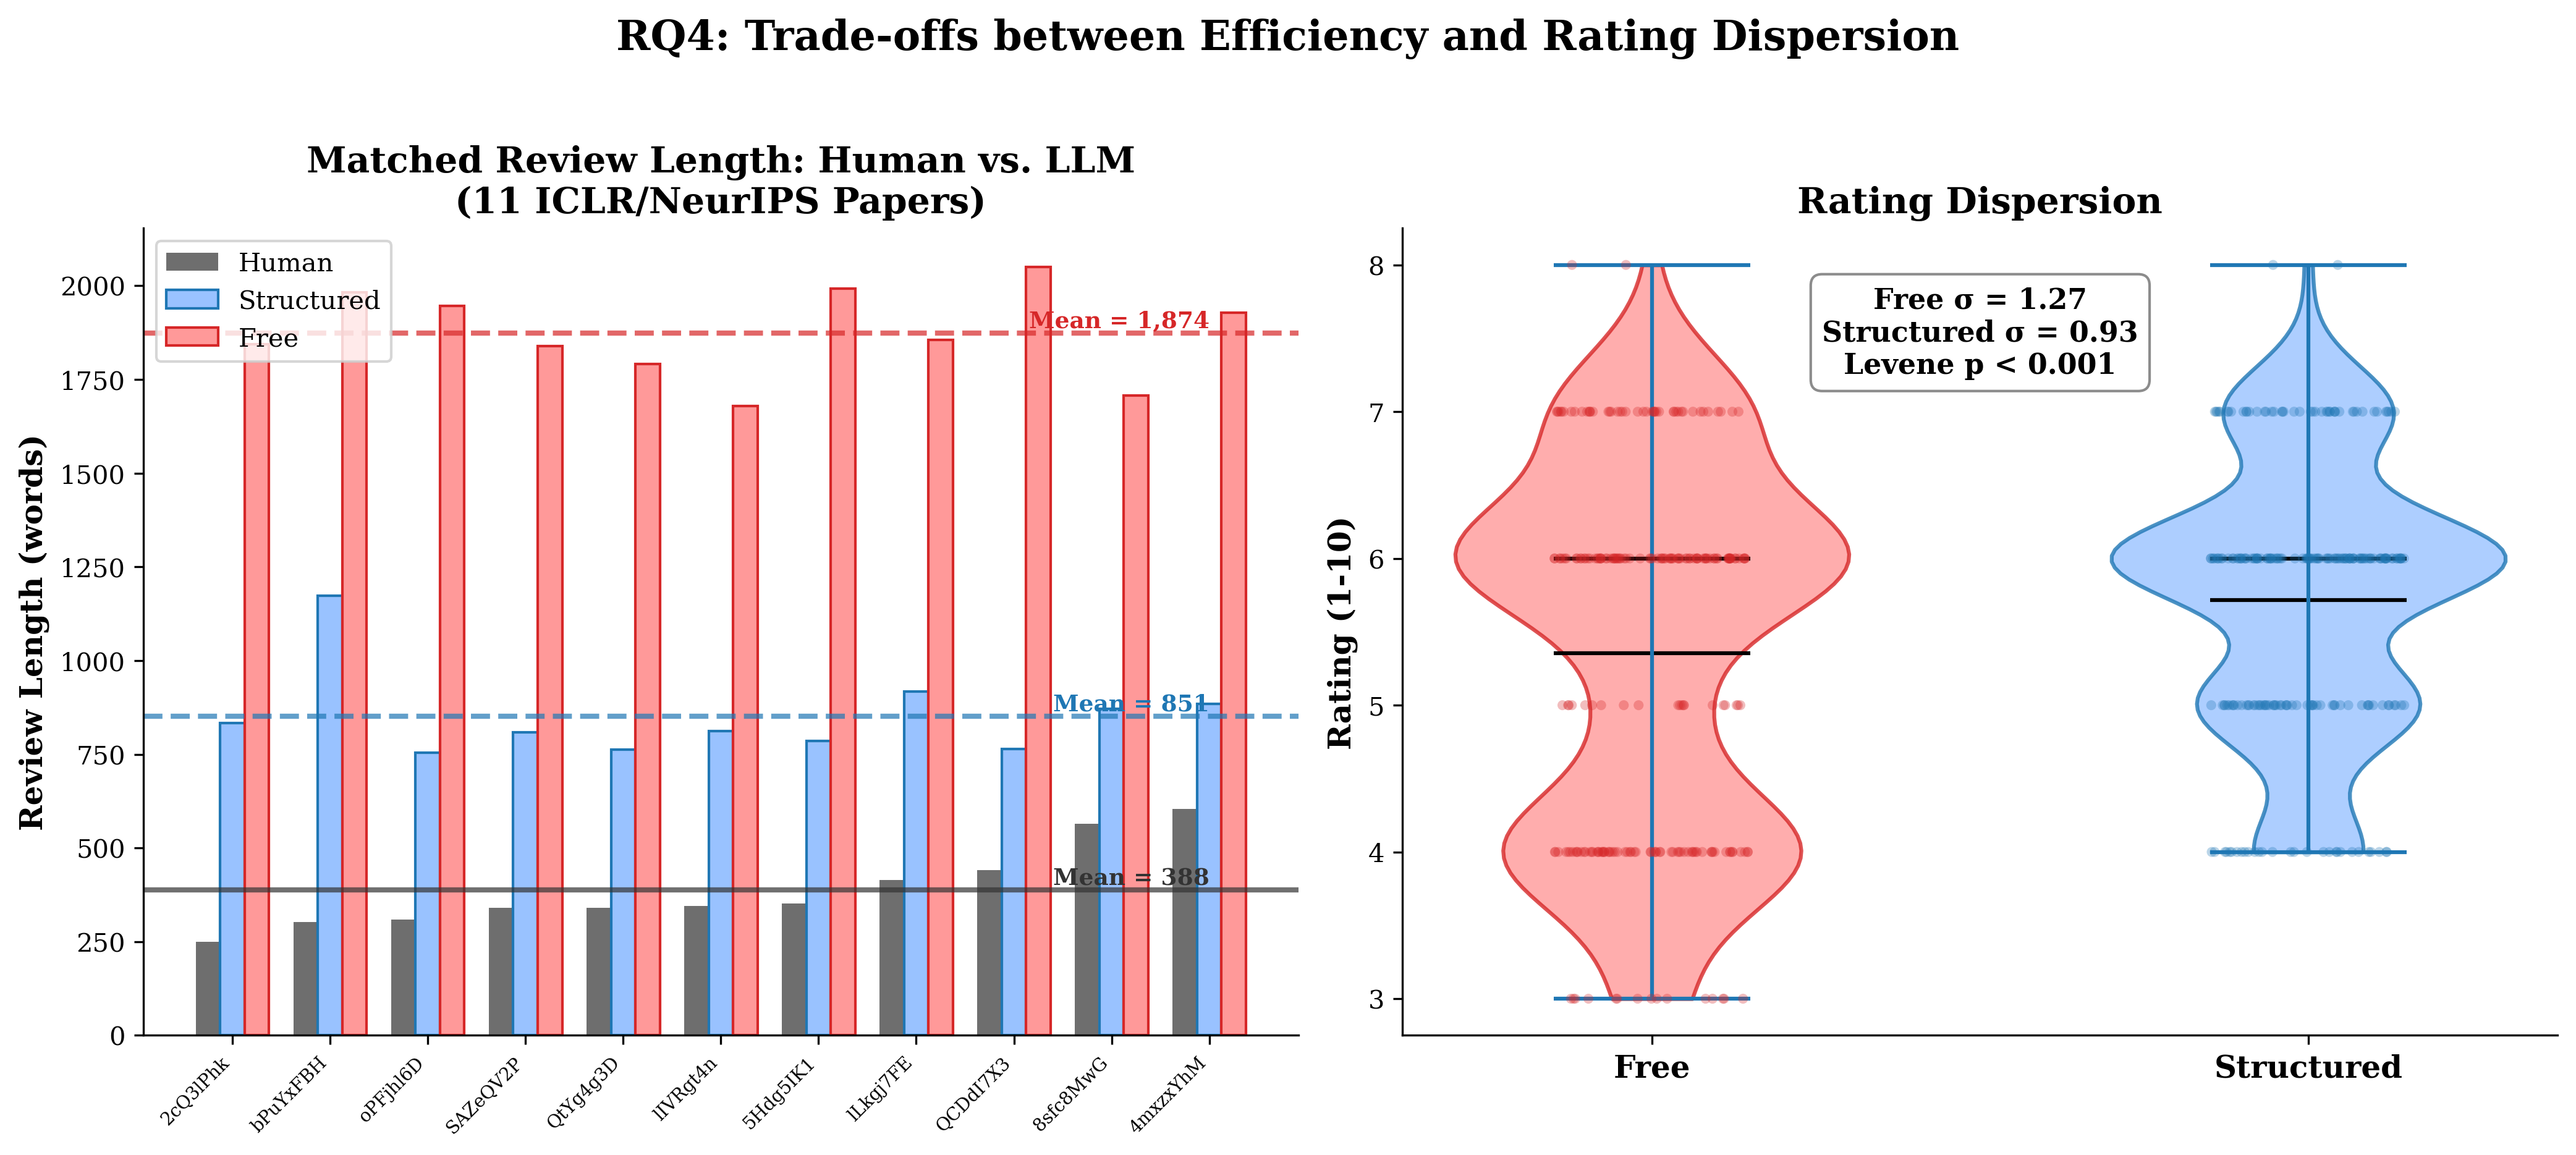
\includegraphics[width=\textwidth]{../../outputs/figures/rq4_tradeoffs.png}
    \caption{Human-relative review length and rating dispersion. Left: matched paper-level mean word counts for 45 Human reviews and the corresponding Original Structured and Free reviews; horizontal lines mark group means. Right: rating distributions across 240 reviews per setup, using Judge-extracted Free ratings and native Structured ratings.}
    \label{fig:rq4-tradeoffs}
\end{figure}

The length benchmark completes the redundancy argument developed in RQ3. Structured reviews were less than half the length of Free reviews while retaining comparable common-coded aspect coverage, and the Human reference was shorter still. Combined with the repeated themes and fine-grained presentation observed in the Free case, these findings provide converging evidence that much of the additional Free output reflects verbosity rather than greater substantive coverage. The aligned reductions in words, latency and tokens establish a clear operational-efficiency advantage for schema-constrained reviewing.

\subsection{Rating Dispersion}
\label{sec:rq4-dispersion}

Structured ratings were less dispersed both globally and within papers. As shown in Table~\ref{tab:rq4-tradeoffs} and the right panel of Figure~\ref{fig:rq4-tradeoffs}, their global standard deviation was 0.93, compared with 1.27 under Free (Levene $p<.001$). Mean within-paper standard deviation was likewise lower at 0.35 versus 0.72, with median values of 0.35 and 0.67, respectively; six papers received an invariant Structured rating across all eight conditions, compared with none under Free. Condition-masked inferred-rating coding reproduced this direction in the auxiliary sample, with standard deviations of 0.53 for Structured and 1.12 for Free.

Exploratory diagnostics did not support the simple explanation that this narrower distribution arose from near-identical review content. The current Structured distribution was not concentrated at a single score, Structured reviews did not exhibit greater token-set overlap, and inspected outputs retained paper-specific summaries and criticisms. The remaining compression may reflect greater consistency, scale compression or reduced sensitivity; the present evidence does not distinguish their relative contributions.

RQ4 therefore shows that schema-constrained reviewing delivered substantial operational and presentational gains: reviews were shorter, faster and less token-intensive, and their length was markedly closer to human reviewing practice. Together with RQ3's comparable common-coded coverage, the human-relative length result supports greater concision without a corresponding coverage loss and reinforces the interpretation that much of the additional Free output was verbose rather than substantively broader. Structured ratings were also more concentrated, but this accompanying distributional difference is not assigned a positive or negative quality interpretation here.

\section{Cross-RQ Synthesis}
\label{sec:results-synthesis}

Taken together, the results position schema-constrained reviewing as a targeted operational control rather than a comprehensive safeguard. Structure attenuated rating inflation, criticism suppression and injection compliance, but did not eliminate manipulation effects. It also failed to improve logic-specific discriminability: target-defect omission remained the primary failure, and detected defects rarely affected the final rating. On secondary performance, Structured reviews achieved comparable common-coded aspect coverage with substantially lower length, latency and token use and were markedly closer to human-review length. Structured ratings were narrower, although the value of this compression remains undetermined. Overall, structure changed the magnitude, distribution and cost of generated reviews and delivered measurable mitigation and concision gains, while reliable input integrity and scientific-logic verification require complementary safeguards.
